\documentclass{standalone}
\usepackage{tikz}

\begin{document}
	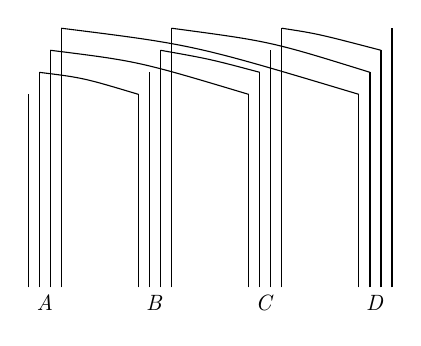
\begin{tikzpicture}[scale=0.7, every node/.style={scale=0.8}]
		
		%Säulen
		\foreach \i in {0,2,4,6} {
			\foreach \j in {0,0.2,0.4,0.6} {
				\draw[thin] (\i+\j,1.5) -- (\i+\j,5+\j*2);
			}
			\node[below] at (\i+0.3, 1.5) {\emph{\char\numexpr65+\i/2}};
		}
		
		
		%Querverbindungen
		\foreach \j in {0.2,0.4,0.6} {
			\draw[thin](\j,5+\j*2) .. controls (\j*5,5+\j*1.5) .. (\j*10,5);
		}	
		
		\foreach \j in {0.4, 0.6} {
			\draw[thin](\j+2,5+\j*2) .. controls ({(\j + 2 + \j*10 + 0.2)/2},5+\j*1.6) .. (\j*10+0.2,5.4);
		}
		
		\draw[thin](4.6,6.2) .. controls (5.25,6.1) .. (6.4,5.8);
		
		%TODO at A terminal
		%		\draw[->] (-1,5.6) -- (0.2,5.4) node[left] at (-1,5.6) {\emph{b}-Kontakt im \emph{A}-Terminal};
	\end{tikzpicture}
\end{document}